\chapter{Diseño e implementación} % Main chapter title

\label{Chapter3} % Change X to a consecutive number; for referencing this chapter elsewhere, use \ref{ChapterX}

\definecolor{mygreen}{rgb}{0,0.6,0}
\definecolor{mygray}{rgb}{0.5,0.5,0.5}
\definecolor{mymauve}{rgb}{0.58,0,0.82}

%%%%%%%%%%%%%%%%%%%%%%%%%%%%%%%%%%%%%%%%%%%%%%%%%%%%%%%%%%%%%%%%%%%%%%%%%%%%%
% parámetros para configurar el formato del código en los entornos lstlisting
%%%%%%%%%%%%%%%%%%%%%%%%%%%%%%%%%%%%%%%%%%%%%%%%%%%%%%%%%%%%%%%%%%%%%%%%%%%%%
\lstset{ %
backgroundcolor=\color{white},   % choose the background color; you must add \usepackage{color} or \usepackage{xcolor}
basicstyle=\footnotesize,        % the size of the fonts that are used for the code
breakatwhitespace=false,         % sets if automatic breaks should only happen at whitespace
breaklines=true,                 % sets automatic line breaking
captionpos=b,                    % sets the caption-position to bottom
commentstyle=\color{mygreen},    % comment style
deletekeywords={...},            % if you want to delete keywords from the given language
%escapeinside={\%*}{*)},          % if you want to add LaTeX within your code
%extendedchars=true,              % lets you use non-ASCII characters; for 8-bits encodings only, does not work with UTF-8
%frame=single,	                % adds a frame around the code
keepspaces=true,                 % keeps spaces in text, useful for keeping indentation of code (possibly needs columns=flexible)
keywordstyle=\color{blue},       % keyword style
language=[ANSI]C,                % the language of the code
%otherkeywords={*,...},           % if you want to add more keywords to the set
numbers=left,                    % where to put the line-numbers; possible values are (none, left, right)
numbersep=5pt,                   % how far the line-numbers are from the code
numberstyle=\tiny\color{mygray}, % the style that is used for the line-numbers
rulecolor=\color{black},         % if not set, the frame-color may be changed on line-breaks within not-black text (e.g. comments (green here))
showspaces=false,                % show spaces everywhere adding particular underscores; it overrides 'showstringspaces'
showstringspaces=false,          % underline spaces within strings only
showtabs=false,                  % show tabs within strings adding particular underscores
stepnumber=1,                    % the step between two line-numbers. If it's 1, each line will be numbered
stringstyle=\color{mymauve},     % string literal style
tabsize=2,	                   % sets default tabsize to 2 spaces
title=\lstname,                  % show the filename of files included with \lstinputlisting; also try caption instead of title
morecomment=[s]{/*}{*/}
}


%----------------------------------------------------------------------------------------
%	SECTION 1
%----------------------------------------------------------------------------------------

Esta sección presenta los detalles técnicos del diseño e implementación de las diferentes funcionalidades del producto, la arquitectura hardware y software, y finalmente la interfaz de usuario para el control y reporte de las operaciones del robot.

El trabajo fue realizado siguiendo una metodología basada en crear un prototipo funcional con una arquitectura escalable que cumpla con alcance básico especificado en el plan de proyecto, y una vez conseguido agregar en lo posible y de acuerdo a la capacidad, funcionalidades adicionales.
De esta forma, una vez que se logró el alcance básico, considerado como la versión v1.0 del producto, se continuó con el desarrollo y se agregó la funcionalidad adicional de control inalámbrico por medio de un joystick, en lo que se considera la versión v2.0 del mismo.

En las siguientes subsecciones se detallan los detalles del diseño e implementación realizados para ambas versiones.


\section{Arquitectura de software del sistema}

Con el fin de poder lograr una arquitectura de software modular, se implementaron diferentes componentes software y servicios que abstraen el acceso a los módulos de hardware (explicados en la siguiente sección) y permite un escalamiento fácil de funcionalidades en la expansión de las funcionalidades del robot entre su versión v1.0 y la v2.0.


\subsection{Arquitectura y diseño de componentes en la versión v1.0}

A continuación se puede apreciar la arquitectura de software del sistema en su versión v1.0 y el detalle de sus componentes y servicios.

\begin{center}
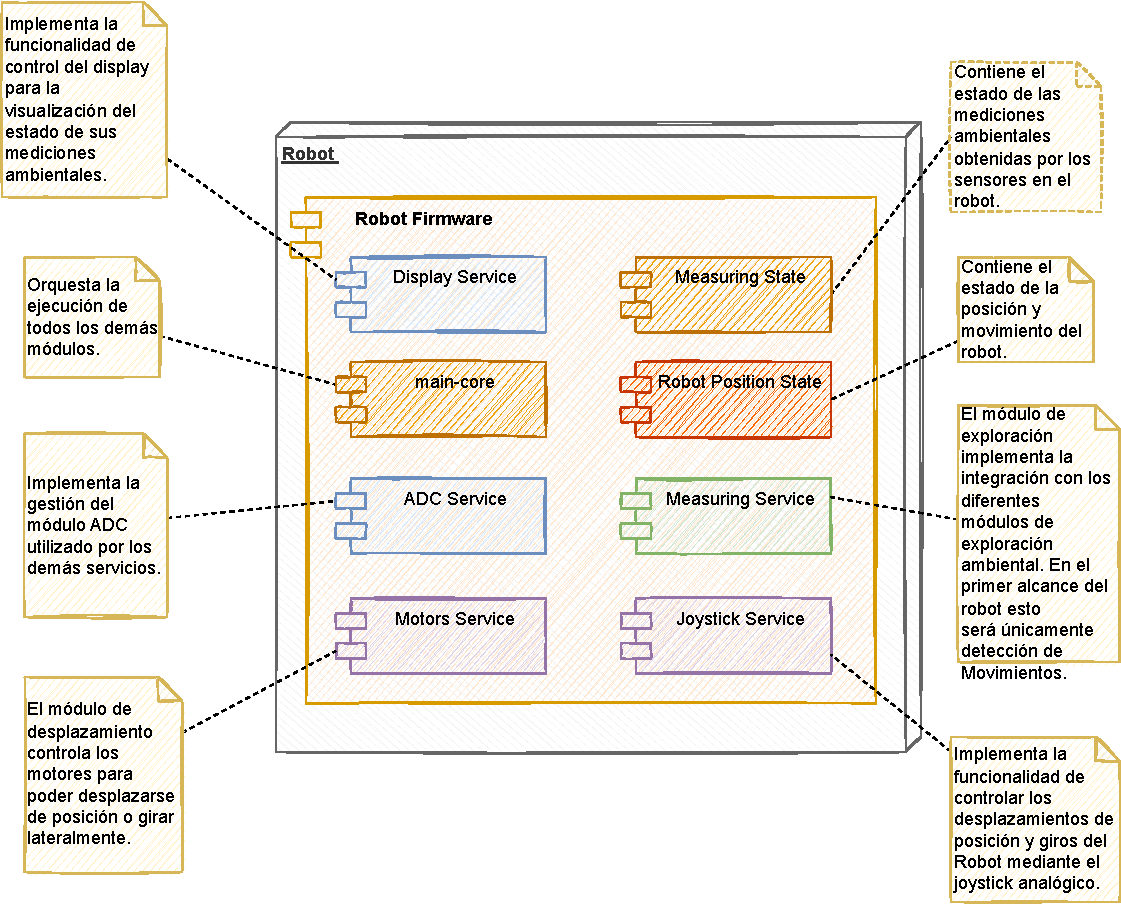
\includegraphics[scale=0.75]{software/arquitectura_software_global_v1}
  \captionof{figure}{Arquitectura global.}
  \label{fig:arquitectura_software_global}

\end{center}


Los componentes y servicios de software del Robot en la versión v1 son los siguientes:

\begin{enumerate}	
	\item Componentes de software
	\begin{enumerate}			
		\item Main-core: orquesta las diferentes tareas desde las que se invocan los demás componentes de software.
		\item Measuring Service: abstrae el acceso a los módulos de medición de temperatura, humedad, presión y luminosidad.
		\item Measuring State: mantiene el estado de cada uno de los parámetros ambientales medidos.
		\item Robot Position State: mantiene el estado del movimiento actual del robot.
		\item ADC Service: abstrae el acceso a los módulos que hacen uso de los canales que requieren conversiones ADC (analógico/digital), como el joystick analógico y el fotorresistor.
		\item Motors Service: abstrae el acceso al módulo de control de motores.
		\item Display Service: abstrae el acceso al módulo de control del display mediante I2C.
		\item Joystick Service: abstrae el acceso al módulo de control del joystick.
	\end{enumerate}	
	\item Servicios (tareas)
	\begin{enumerate}				
		\item Display Task	
		\item Measuring Task		
		\item Joystick Task
		\item Motors Task		
	\end{enumerate}			
\end{enumerate}		

\subsection{Arquitectura y diseño de componentes en la versión v2.0}

Luego de expandir su funcionalidad, los componentes y servicios de software se separaron físicamente en el hardware del robot y el del joystick, agregando además los necesarios para la comunicación inalámbrica. A continuación se puede apreciar la arquitectura de software del sistema en su versión v2.0 y el detalle de sus componentes y servicios.

\begin{center}
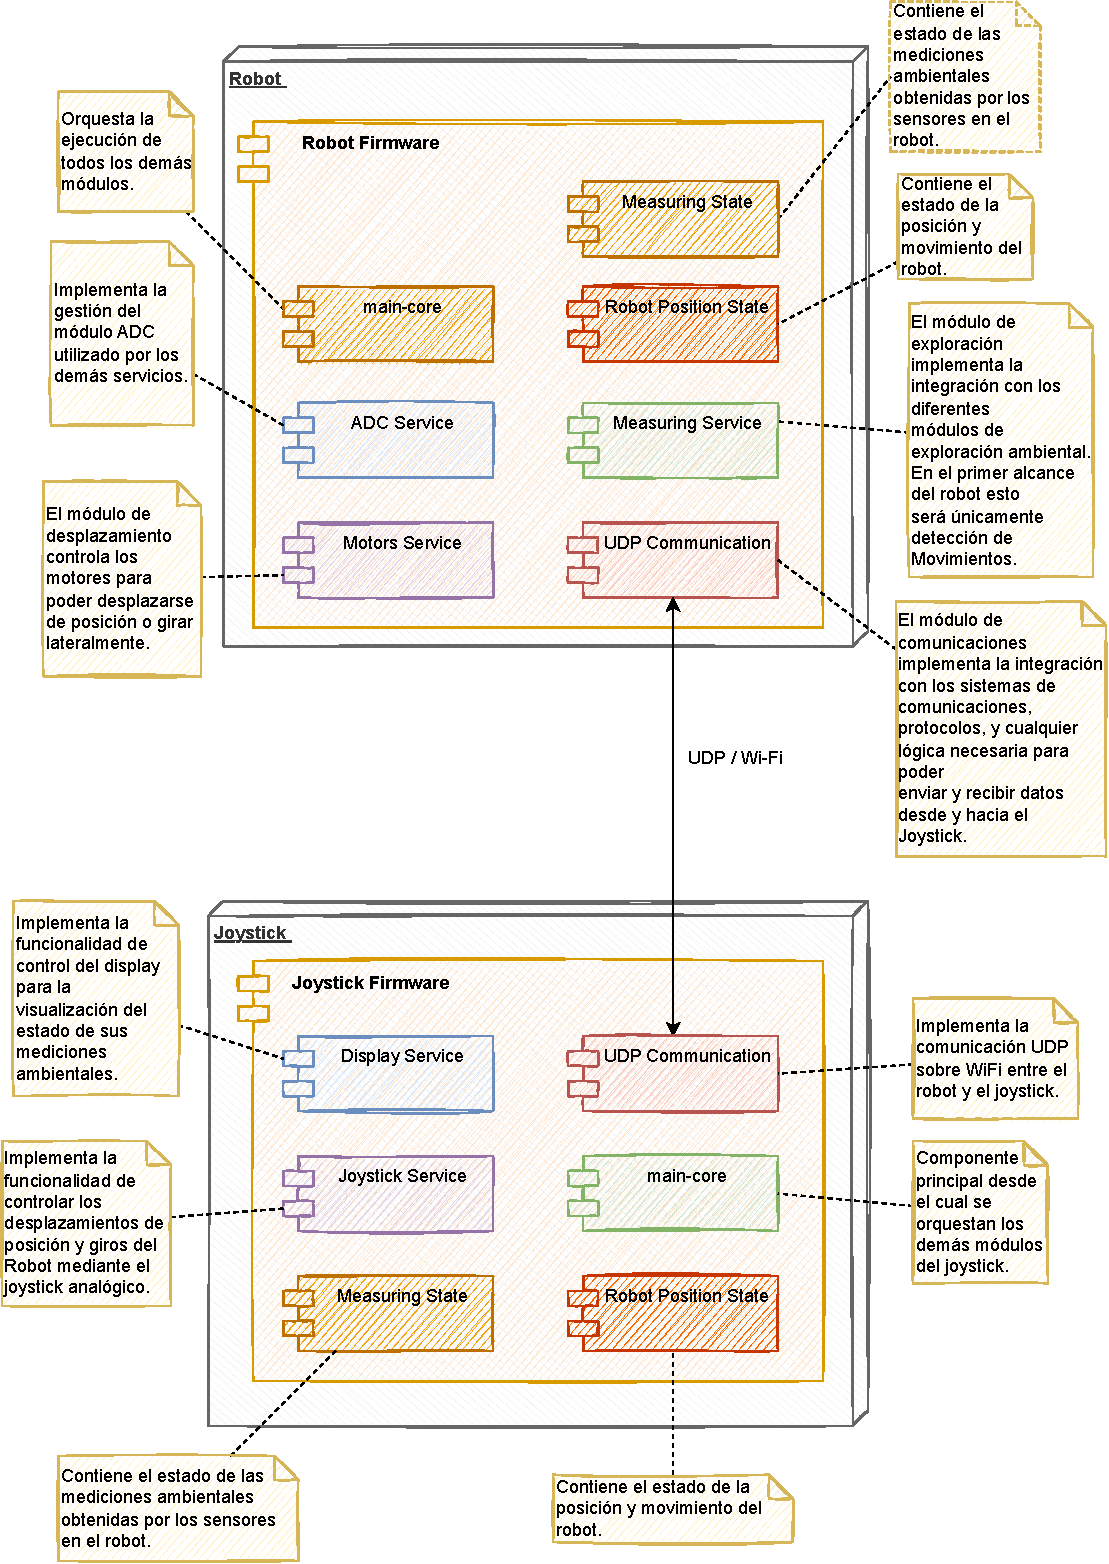
\includegraphics[scale=0.75]{software/arquitectura_software_global_v2}
  \captionof{figure}{Arquitectura global.}
  \label{fig:arquitectura_software_global}

\end{center}

Los componentes de software y servicios del robot son:

\begin{enumerate}	
	\item Componentes de software
	\begin{enumerate}			
		\item Main-core
		\item Measuring Service	
		\item Measuring State
		\item Robot Position State
		\item ADC Service
		\item Motors Service
		\item WIFI Service
		\item UDP Service	
	\end{enumerate}	
	\item Servicios (tareas)
	\begin{enumerate}				
		\item Measuring Task		
		\item Motors Task	
		\item UDP Server Task
	\end{enumerate}			
\end{enumerate}		


Los componentes de software y servicios del joystick son:

\begin{enumerate}	
	\item Componentes de software
	\begin{enumerate}			
		\item main-core
		\item Measuring State
		\item Robot Position State
		\item UDP Service	
	\end{enumerate}	
	\item Servicios (tareas)
	\begin{enumerate}				
		\item Display Task		
		\item Joystick Task	
		\item UDP Server Task
	\end{enumerate}			
\end{enumerate}		

\section{Implementación de los módulos}

Los macro componentes de hardware presentes en la arquitectura de la versión v2.0 son el robot y el joystick, que constituyen dos sistemas embebidos independientes implementados con dos microcontroladores ESP32, integrados entre sí por medio de una red WiFi y una comunicación UDP. La arquitectura de hardware del sistema esta compuesta por los siguientes módulos:


\begin{itemize}
	\item En el robot:
	\begin{itemize}
		\item Control de los motores DC.	
		\item Control de los sensores de medición (DHT11, BMP280 y fotorresistor).
		\item Gestión de la  comunicación inalámbrica vía Wi-Fi (en la versión v2.0).
	\end{itemize}
	\item En el joystick:
	\begin{itemize}
		\item Control del display.
		\item Control del joystick.
		\item Gestión de la  comunicación inalámbrica vía Wi-Fi (en la versión v2.0).
	\end{itemize}
\end{itemize}

La integración de los mismos se realizó mediante el diseño y construcción de una placa integradora central, que conecta los dispositivos hardware con el microcontrolador ESP-32.


\subsection{Control de la red Wi-Fi}

El módulo de red WiFi está integrado en el chip ESP32, el cual soporta múltiples características \cite{ESP32_WiFi} por lo tanto a nivel hardware no fue necesario realizar ningún conexionado.
A nivel de software, la gestión del módulo WiFi está incluida en el SDK ESP-IDF, y el acceso a este se realiza desde el módulo ADC 2 \cite{ESP32_adc}. Por este motivo, cuando el sistema embebido utiliza el módulo WiFi, el uso del ADC2 queda restringido a esta funcionalidad por lo tanto cualquier otro dispositivo que deba hacer uso del ADC debe ser configurado para utilizar el ADC1, como en el caso de los módulos de joystick y detección de luminosidad, que se explican en las siguientes secciones.

La configuración del \textit{soft access point Wi-Fi} implementado se realizó en base a los parámetros de red detallados en la siguiente tabla  \ref{tab:configuracion_wifi}:

\vspace{0.5cm}
\begin{table}[h]
\centering
\caption[Configuración de AP WiFi]{Configuración de AP WiFi}
\begin{tabular}{l c c}
\toprule
\textbf{Parámetro} & \textbf{Valor} \\
\midrule
SSID & Robot  \\
Password & Robot  \\
\bottomrule
\hline
\end{tabular}
\label{tab:configuracion_wifi}
\end{table}


El desarrollo de este módulo se basó en el ejemplo provisto por Espressif \cite{ESP32_WiFi_SoftAP}. El código fuente del prototipo realizado puede apreciarse en el siguiente enlace \cite{ESP32_POC_WiFi}.


\subsection{Control del joystick analógico}
Para el desarrollo de este prototipo se utilizó el SDK ESP-IDF y se configuró el módulo ADC1 de acuerdo a los siguientes detalles en la tabla \ref{fig:conexionado_joystick}:

\vspace{0.5cm}
\begin{table}[h]
\centering
\caption[Conexionado joystick]{Conexionado joystick.}
\begin{tabular}{l c c}
\toprule
\textbf{Channel} & \textbf{Unit} & \textbf{Pin GPIO}\\
\midrule
6 & 1 & 34 \\
7 & 1 & 35 \\
\bottomrule
\hline
\end{tabular}
\label{tab:conexionado_joystick}
\end{table}

A continuación, se puede apreciar el conexionado físico en la figura \ref{fig:conexionado_joystick}.

\begin{center}
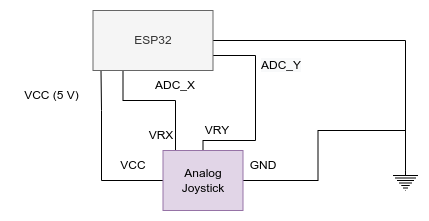
\includegraphics[scale=1]{schematics/conexionado_joystick}
  \captionof{figure}{Conexionado joystick.}
  \label{fig:conexionado_joystick}
\end{center}


El desarrollo de este módulo se basó en el ejemplo provisto por Espressif \cite{ESP32_ADC1_Example}. El código fuente del prototipo realizado puede apreciarse en el siguiente enlace \cite{ESP32_POC_joystick}.


\subsection{Medición de valor de luminosidad}
Debido a su fuerte dependencia con la temperatura, y especialmente a que su distribución espectral no resulta adecuada para la medición de iluminancia, los fotoresistores no pueden proporcionar una medición precisa de iluminancia como lo haría un luxómetro. No obstante, el fotorresistor resulta puede ser utilizado como sensor para proporcionar medidas cuantitativas sobre el nivel de luz, tanto en interiores como en exteriores.
Para leer los valores del fotorresistor se utilizó la función \textbf{adc1\textunderscore get\textunderscore raw } del SDK ESP-IDF, donde el valor devuelto se encuentra en el rango [0 - 2050], con \textit{\textbf{0}} el valor de mayor iluminación y \textit{\textbf{2050}} el menor.
Finalmente, para calcular el nivel de iluminación como valor porcentual, en el rango [0-100], siendo cero el nivel más oscuro y cien más iluminado, se utilizó la siguiente función matemática:

\begin{equation*}
\mbox{Nivel de Iluminación}=\frac{\mbox{MaxReading - reading}}{\mbox{MaxReading}} x 100
\end{equation*}

Donde:
\begin{itemize}
	\item El valor \textit{reading} es la lectura analógica del valor del fotorresistor.
	\item El valor \textit{MaxReading} es el máximo valor analógico posible de ser entregado por el fotorresistor, en este caso 2050.
	\item El valor \textit{MaxReading} es el máximo valor analógico posible de ser entregado por el fotorresistor, en este caso 0.
\end{itemize}

Para el desarrollo de este prototipo se utilizó el SDK de ESP-IDF y se configuró el módulo ADC1 de acuerdo a los detalles provistos en la tabla \ref{tab:conexionado_fotoresistor}.

\vspace{0.5cm}
\begin{table}[h]
\centering
\caption[Conexionado fotoresistor]{Conexionado fotorresistor.}
\begin{tabular}{l c c}
\toprule
\textbf{Channel} & \textbf{Unit} & \textbf{Pin GPIO}\\
\midrule
0 & 1 & 36 \\
\bottomrule
\hline
\end{tabular}
\label{tab:conexionado_fotoresistor}
\end{table}

A continuación, se puede apreciar un diagrama de su conexionado físico en la figura \ref{fig:conexionado_fotoresistor}.

\begin{center}
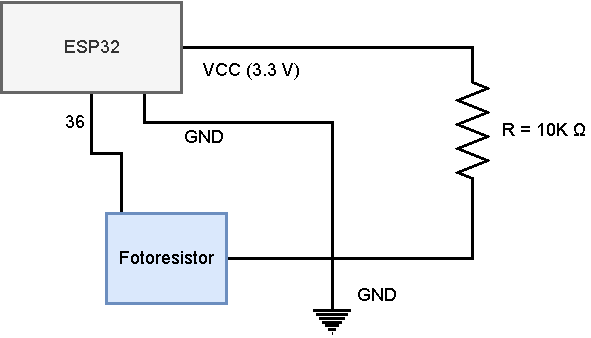
\includegraphics[scale=1]{schematics/conexionado_fotoresistor}
  \captionof{figure}{Conexionado fotorresistor.}
  \label{fig:conexionado_fotoresistor}
\end{center}

El desarrollo de este módulo se basó en el ejemplo provisto por Espressif \cite{ESP32_ADC1_Example}. El código fuente del prototipo realizado puede apreciarse en el siguiente enlace \cite{ESP32_POC_photoresistor}.

\subsection{Medición de temperatura y humedad}

Para el desarrollo de este modulo se utilizó la biblioteca de código ESP-IDF-Lib Components Library \cite{esp_idf_lib_website} que provee el soporte para gestionar el DHT11. Para acceder a las lecturas del dispositivo se abstrajo mediante el componente Measuring Service, este es invocado por la tarea Measuring Task y el estado de la lectura es almacenado en el componente Measuring State.
A continuación, se puede apreciar el conexionado del prototipo en la figura \ref{fig:conexionado_dht11}.

\begin{center}
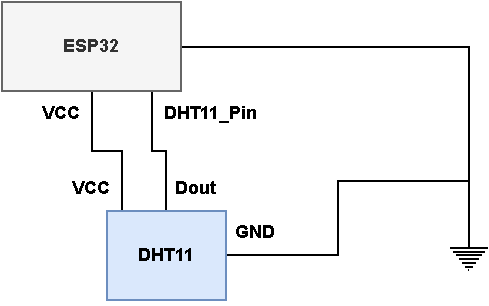
\includegraphics[scale=1]{schematics/conexionado_dht11}
  \captionof{figure}{Circuito del conexionado DHT11.}
  \label{fig:conexionado_dht11}
\end{center}

El desarrollo de este módulo se basó en el ejemplo provisto por la biblioteca ESP-IDF-Lib \cite{ESP32_dht11_example}. El código fuente del prototipo realizado puede apreciarse en el siguiente enlace \cite{ESP32_POC_dht11}.

\subsection{Medición de presión}
Para el desarrollo de este módulo se utilizó el framework ESP-IDF y la biblioteca de código ESP-IDF Components que provee el soporte para gestionar el dispositivo BMP280 por medio del protocolo I2C. El driver es inicializado en el componente main-core para ser posteriormente invocado desde el Measuring Service en la tarea Measuring Task. Sus lecturas son guardadas en el Measuring State. A continuación, se puede apreciar el conexionado del prototipo en la figura \ref{fig:conexionado_bmp280}.
\begin{center}
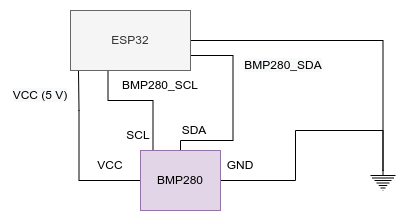
\includegraphics[scale=1]{schematics/conexionado_bmp280}
  \captionof{figure}{Conexionado BMP280.}
  \label{fig:conexionado_bmp280}
\end{center}

El desarrollo de este módulo se basó en el ejemplo provisto por la biblioteca ESP-IDF-Lib \cite{ESP32_bmp280_example}. El código fuente del prototipo realizado puede apreciarse en el siguiente enlace \cite{ESP32_POC_bmp280}.


\subsection{Control de motores DC}

Para la implementación del módulo de control de los motores de corriente continua se utilizaron a nivel de hardware dos módulos puentes L298N \cite{L298N}, que permiten integrar y controlar dos motores cada uno. Con el fin de alimentar los módulos con una fuente de poder de corriente y tensión consistente, se utilizaron dos baterías de Li-Ion de 3,7 V y 2000 mA/h conectadas en serie, activadas mediante un interruptor.
A nivel driver en el ESP32 se utilizó el módulo de control de motores por modulación de pulsos (MCPWM) \cite{ESP32_MCPWM} que por medio de la configuración de sus unidades y del \textit{duty cycle} \cite{ESP32_MCPWM_2} se puede controlar el sentido y velocidad de rotación de los motores.
Los puentes L298N proporcionan también además una tensión de salida de 5 V, y que se utilizó para la alimentación del ESP32 conectando su pin Vin.

En el siguiente diagrama puede apreciarse el conexionado lógico para el control de los motores con los componentes mencionados.

\begin{center}
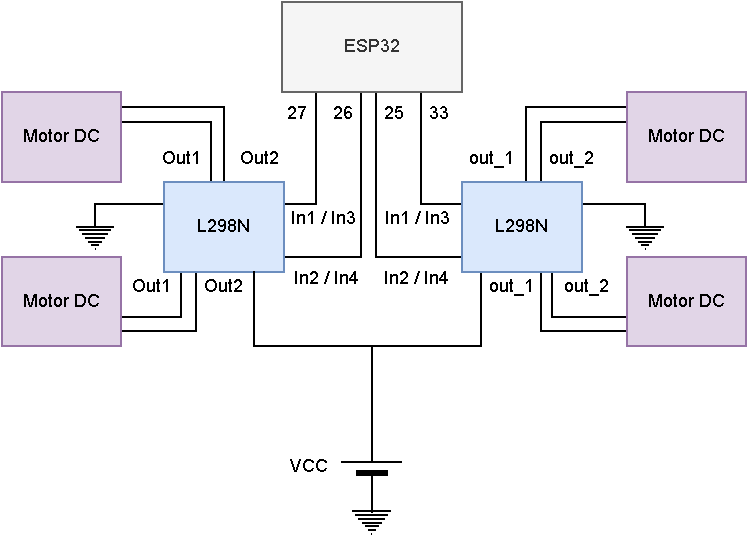
\includegraphics[scale=1]{schematics/conexionado_motores}
  \captionof{figure}{Conexionado motores.}
  \label{fig:conexionado_motores}
\end{center}

El desarrollo de este módulo se basó en el ejemplo provisto por Espressif \cite{ESP32_MCPWM_example}. El código fuente del prototipo realizado puede apreciarse en el siguiente enlace \cite{ESP32_POC_motor_MCPWM}.



\subsection{Control del display}

Para la implementación del módulo de visualización de valores observados se integró un display de dos líneas y dieciséis caracteres LCM1602A por medio de un driver I2C que facilita su control. Al basarse en el protocolo I2C el display comparte las mismas líneas SCL y SDA que el sensor BMP280.

\begin{center}
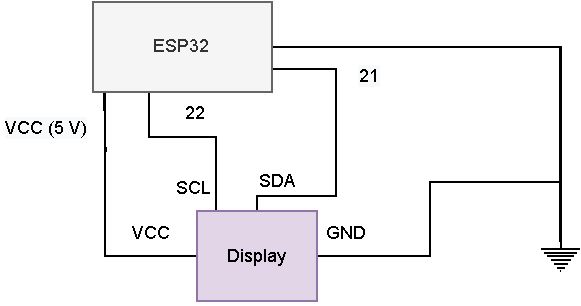
\includegraphics[scale=1]{schematics/conexionado_display}
  \captionof{figure}{Conexionado display.}
  \label{fig:conexionado_display}

\end{center}


El desarrollo de este módulo se basó en el ejemplo provisto en el enlace \cite{ESP32_Display_Example}. El código fuente del prototipo realizado puede apreciarse en el siguiente enlace \cite{ESP32_POC_display}.


\section{Arquitectura de hardware}


\subsection{Ensamblado final del producto v2.0}

En las siguientes imagenes se pueden apreciar las diferentes perspectivas del robot y del joystick.

\begin{center}
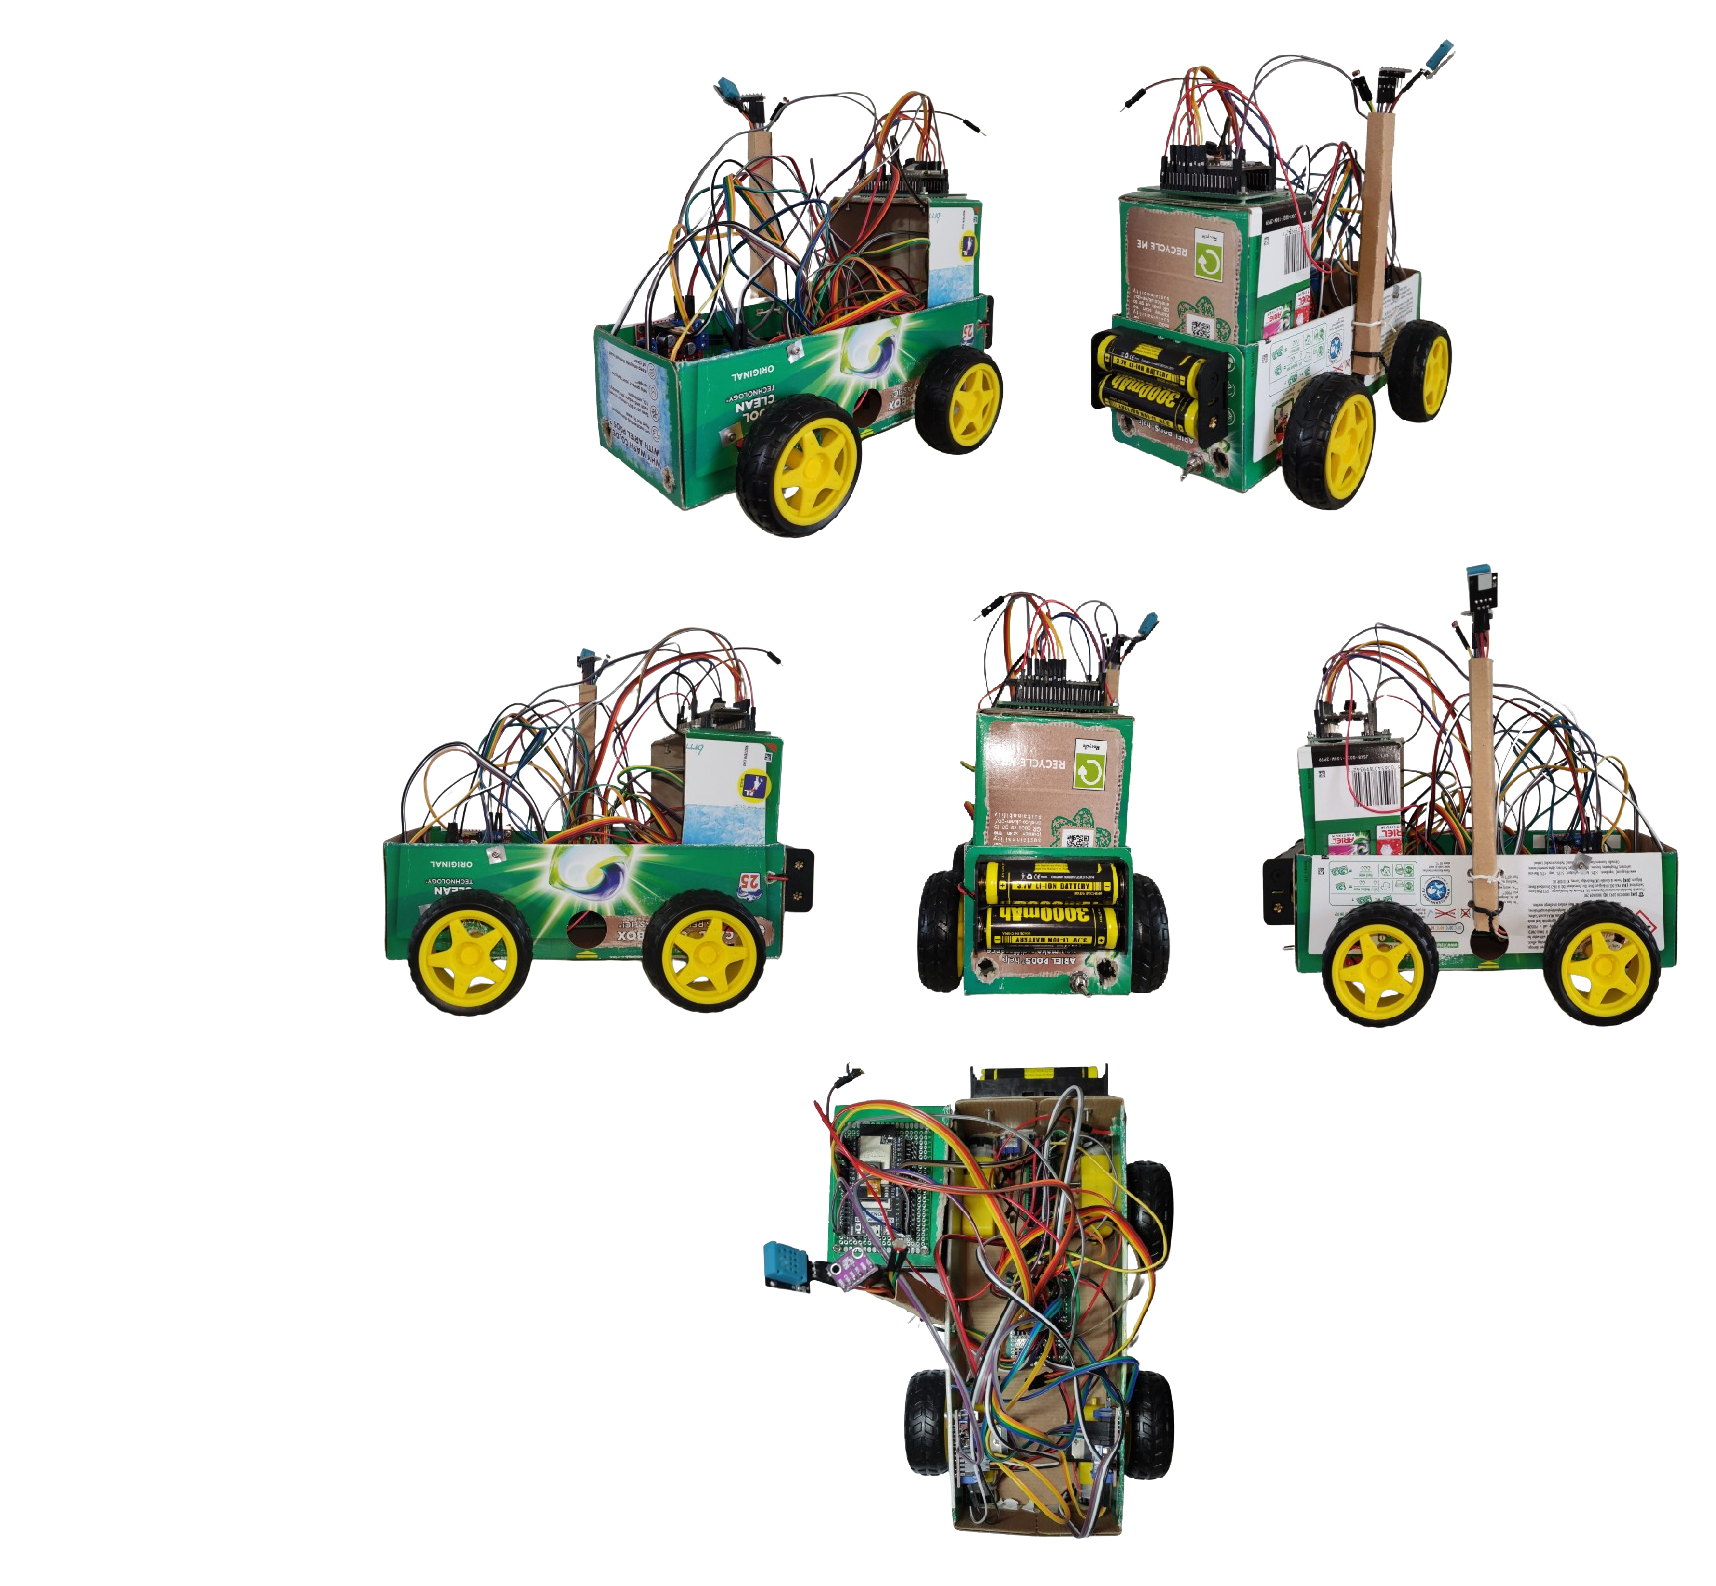
\includegraphics[scale=0.5]{demo_product/all_perspectives_robot}
  \captionof{figure}{Hardware del robot.}
  \label{fig:conexionado_fisico}
\end{center}


\begin{center}
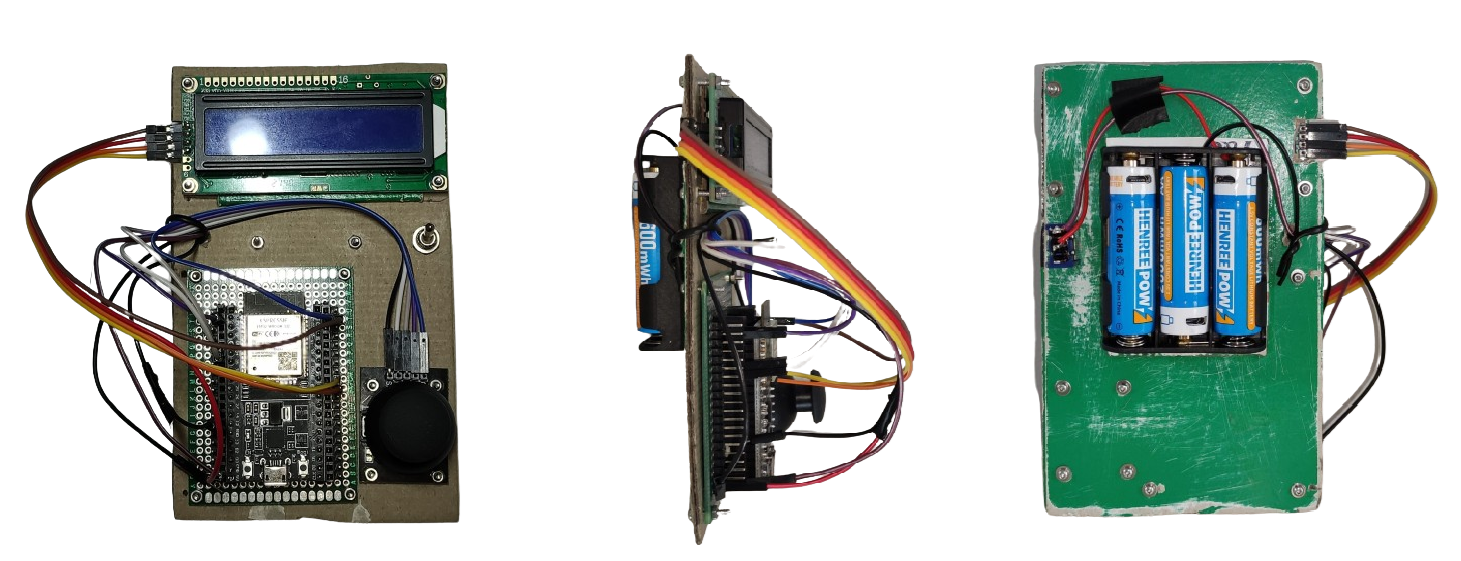
\includegraphics[scale=0.55]{demo_product/all_perspectives_joystick}
  \captionof{figure}{Hardware del joystick.}
  \label{fig:conexionado_fisico}
\end{center}



\subsection{Conexionado lógico }

En las siguientes imagenes se pueden apreciar los conexionados lógicos del robot y del joystick.

\begin{center}
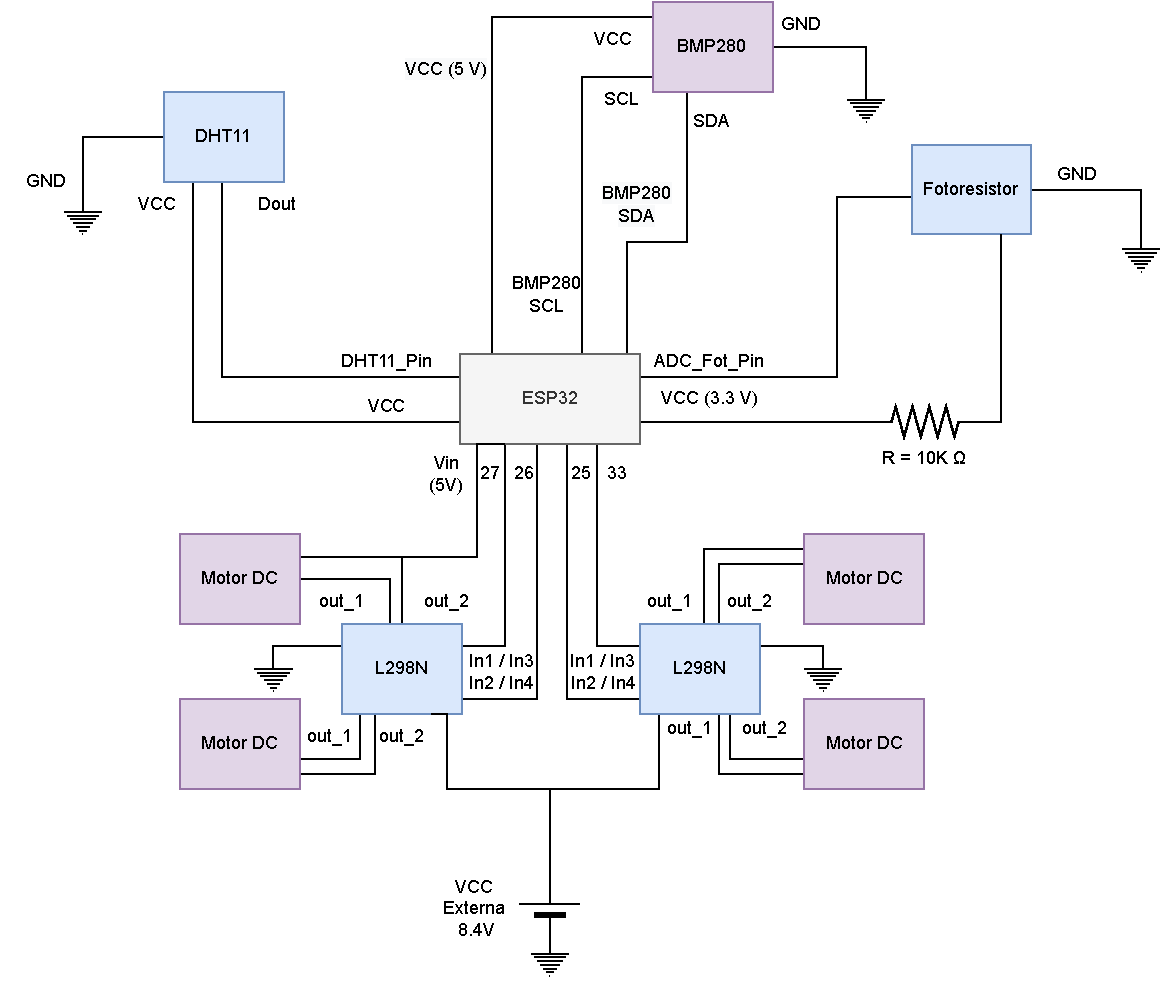
\includegraphics[scale=0.75]{schematics/conexionado_completo_robot}
  \captionof{figure}{Conexionado del robot.}
  \label{fig:conexionado_completo_robot}
\end{center}


\begin{center}
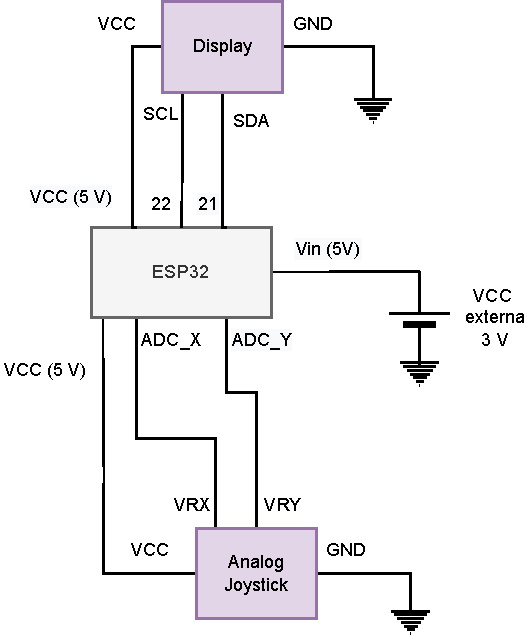
\includegraphics[scale=0.75]{schematics/conexionado_completo_joystick}
  \captionof{figure}{Conexionado del joystick.}
  \label{fig:conexionado_completo_joystick}
\end{center}


\subsection{Conexionado físico}

En la siguiente imagen se puede apreciar el conexionado fisico del robot.

\begin{center}
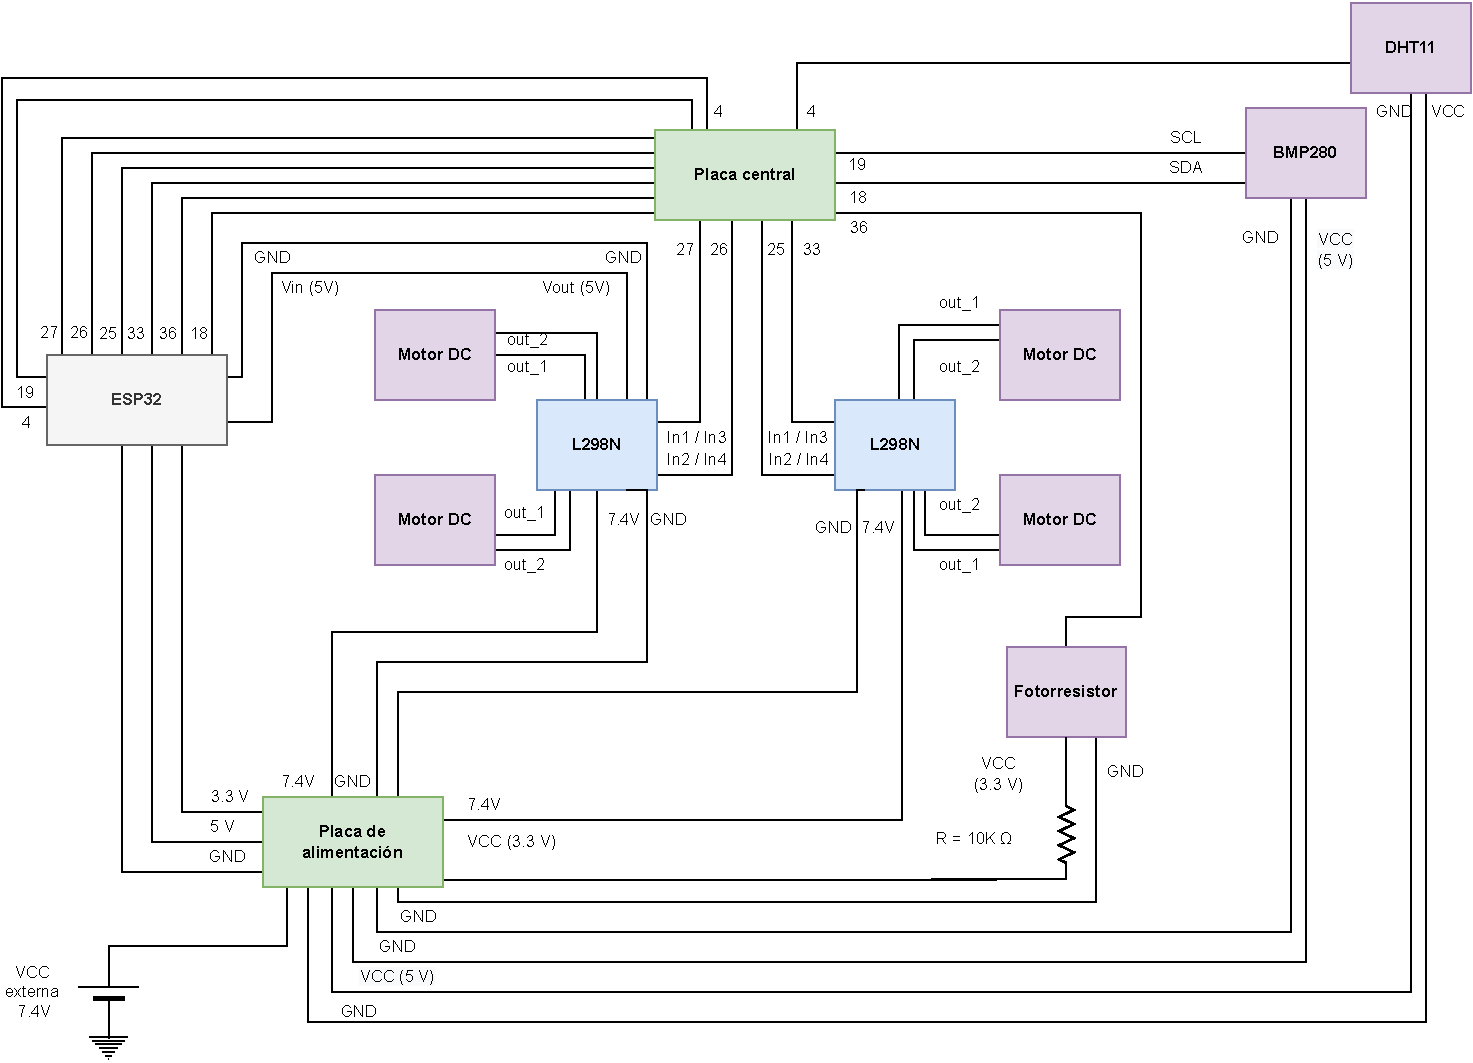
\includegraphics[scale=0.6]{schematics/conexionado_fisico}
  \captionof{figure}{Conexionado físico del robot.}
  \label{fig:conexionado_fisico}
\end{center}




\section{Ciclo de desarrollo}

Durante el ciclo de desarrollo se utilizaron las herramientas explicadas en el capítulo anterior, y se creó por cada prototipo una imagen Docker extendiendo la de espressif/idf \cite{Espressif_docker_image}. El proceso de compilación y despliegue está explicado en la documentación técnica del producto \cite{Robot_Tecnical_doc}.










